%************************************************
\chapter{About Dorel Industries}
\label{chp:about}
%************************************************
\section{Introduction}
\index{History}In 1962, Leo Schwartz founded "Dorel Co. Ltd" in Quebec, and began producing juvenile products.  It was not until 1962 that "Dorel Co. LTD" became "Dorel Industries", following a merger with Ridgewood Industries (a furniture manufacturing company).  Since then, the company has continued to grow primarily through acquisitions, eventually branching out to the recreational and leisure markets by acquiring Schwinn and Cannondale \cite{DorelIndustries2013}.

\section{History}


\section{Recent Strategic Moves}\index{Recent Strategic Moves}
\begin{itemize}
  \item (2013) Dorel began a massive share buyback plan in order to raise its market value \cite{Smith2014}.
  \item (2013) The company acquired a 70\% controlling interest in Caloi (a major brazilian bicycle manufacturer).  This acquisition is intended to help Dorel expand into Latin America, as Caloi is the number one bicycle brand in the region \cite{DorelIndustries2013}.
  \item (2013) Dorel’s assembly and testing facilities located in \index{Bedford, PA}Bedford, PA are being shut down and relocated overseas in an effort to reduce expenses \cite{VoiceofAmerica2009}.
  \item (2012) Dorel began sponsoring the newly created \index{Cannondale Pro Cycling Team}"Cannondale Pro Cycling Team", in order to increase brand exposure \cite{DorelIndustries2012} .
\end{itemize}







%************************************************
\chapter{Corporate Strategy Analysis}
\label{chp:corporatestrategy}
%************************************************

\section{Business Definition}

Dorel Industries has a diverse business definition.   Dorel makes high quality furniture, juvenile and recreational products for consumers who emphasize quality and durable products.  Dorel’s technologies include ready-to-assemble furniture, high quality durable bicycles as well as safe and reliable baby products \cite{DorelIndustries2013}.

Dorel’s business is comprised of several very distinct products amongst completely unrelated markets. Dorel’s \index{Main Products}main products include furniture, bicycles and baby products.  These products relate to Dorel’s business units.   In term’s of Dorel’s target markets, the United States has traditionally been a very important market. However, due to the US economy downturn, Dorel has began focusing on extending their business internationally.  Lastly, the technology that Dorel institutes is one of outsourcing manufacture of their products, in order to be able to compete on price, specifically for their home furnishings business unit.

One of the primary issues with this business definition is that there does not appear to be much \index{Synergy}synergy among the product lines. The manufacture of the products, the products themselves, and the target markets of each product are all wholly unrelated. As part of our recommendation, Dorel would benefit from finding a way to make themselves more internally consistent.

\begin{itemize}        	
  \item Products
    \begin{itemize}
      \item Furniture
      \item Bicycles
      \item Baby products/accessories
    \end{itemize}
  \item Markets (respectively)
    \begin{itemize}     
      \item North American retail chains
      \item Mass merchant / Independent Bike Dealer (IBD) network
      \item US and International retail chains
    \end{itemize}
  \item Technology
    \begin{itemize}     
      \item Ready-to-assemble furniture
      \item High Quality products
      \item Safe and durable juvenile products
    \end{itemize}
\end{itemize}


\section{Business Unit Breakdown}
Dore’s business is comprised of 3 distinct business units; Juvenile, Home Furnishings and Recreational/Leisure.  These 3 business units drove 2012 revenue of \$2.49 Billion, as well as \$583 Million in gross profit. A breakdown of each business unit follows.

\subsection{Juvenile}
The \index{Juvenile}Juvenile business unit is focused on the manufacture and import of high quality, safe and fashionable juvenile products.  These products include car seats, strollers, high chairs, etc.  Products are provided under their own brand names, as well as house brand names for their customers. This segment produced 2012 revenues of \$1.04 Million, which equates to 42\% of the business. This segment produced \$287 Million in \index{Gross Profit}gross profit which was 49\% of Dorel’s total gross profit.

Dorel is focusing on growing this segment in Latin America, where the retail environment is beginning to prosper and birthrates in this region are an incline. Dorel has also made very recent \index{Acquisitions}{acquisitions for this segment to expand its breadth of offering as well as introduction to new international channels.

\subsection{Recreational/Leisure}
The \index{Recreational/Leisure}Recreation/Leisure business is comprised of premium/mass market bicycles, jogging strollers, ride-on toys as well as branded performance apparel.  This segment has a focus on international markets, with 50\% of sales coming from the Asia-Pacific region (US accounts or 12\%). This segment accounted for 37\% of Dorel’s 2012 revenue, or \$928 Million, with gross profit at \$233 Million.

Dorel is focused on making this segment the premier bicycle business in the market. in 2012, \index{Expenses}selling expenses for this business unit increased 13\%, which leadership attributed to \index{Marketing}marketing efforts to enrich this segment’s brands.

\subsection{Home Furnishings}
\index{Home Furnishings}The Home Furnishings business focuses on ready-to-assemble furniture, step stools, futons and imported home entertainment furniture.  The primary focus for this segment is North American markets, which is evident since Dorel has five distinct segments within this business unit. This segment drove 21 percent of Dorel’s 2012 revenue with \$521 million, as well as 11% of gross profit with \$62 million

This segment is the \index{Cash Cow}cash cow for Dorel.  However, with this segment’s focus being on the North American market, home-related market, this segment has suffered a bit with the \index{US Economy}US economy.  Recenty, Dorel moved more of its manufacturing overseas, which should help with this segment’s ability to compete on price in their mass retail chains.

\begin{table}[h]
    \begin{tabular}{lllllllllll}
    {\bf \underline{Unit}}                 & {\bf \underline{Total Sales}}    & {\bf \underline{\%}}  & {\bf \underline{Gross Profit}} & {\bf \underline{\%}}\\
    Juvenile             & \$1,040,765,000 & 42\% & \$287,658,000 & 49\% \\
    Home Furnishings     & \$521,523,000  & 21\% & \$62,552,000 & 11\% \\
    Recreational/Leisure & \$928,422,000  & 37\% & \$233,437,000 & 40\% \\
    \end{tabular}
\end{table}

\begin{table}[h]
    \begin{tabular}{lllllllllll}
    {\bf \underline{Unit}}             &  {\bf \underline{Operating Profit}} & {\bf \underline{\%}}  & {\bf \underline{Unit Strength}} & {\bf \underline{Industry Potential}} \\
    Juvenile             & \$73,313,000     & 43\% & 3 & 4 \\
    Home Furnishings     & \$25,593,000     & 15\% & 1 & 2 \\
    Recreational/Leisure  & \$71,958,000     & 42\% & 4 & 2 \\
    \end{tabular}
\end{table}
%----------------------------------------------------------
%************************************************
\section{Modified BCG}
\label{chp:bcg}
%************************************************
\centerline{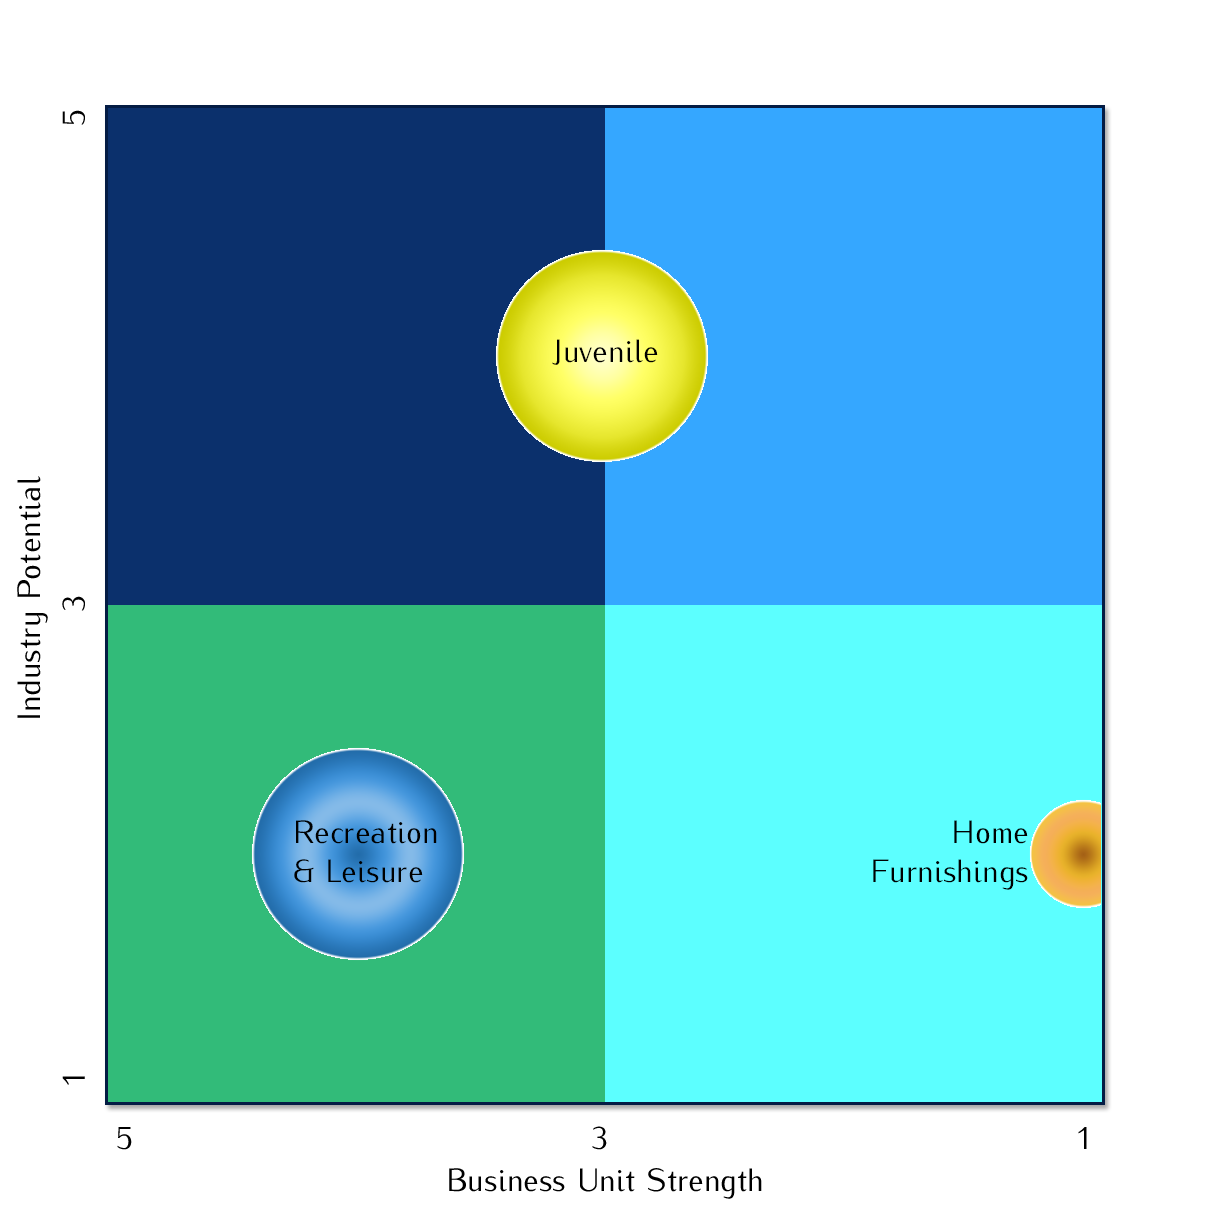
\includegraphics[scale=0.5]{BCG}}
\paragraph{NOTE:}\index{BCG}Market growth rate/market share is in comparison to Dorel’s primary competitor in each division.  (Recreational/Leisure compared with Huffy Corporation, Juvenile to Kid Brands, Inc. and Home Furnishings compared with IKEA).  Because there are other unaccounted for competitors (privately owned, unable to obtain financials), it is likely that all 3 divisions are actually lower on the graph than shown here.  It is unlikely that any of the units are actually approaching “Star” status.  Additionally, the size of each circle is relative in proportion to the percentage of revenue that it is bringing into Dorel.
\subsection{BCG Analysis}
This BCG graph illustrates some of Dorel's current issues.  After accounting for market share being lower than shown, the Juvenile unit is at best a \index{Cash Cow}slowly dying cash cow, trending towards \index{Dog}dog territory.  The recreational/leisure unit is questionable, but has the potential to be a \index{Star}star.  And lastly, the furnishings unit may be growing quickly, but is currently bringing in the smallest amount of \index{Revenue}revenue.
%---------------------------------------------------------------

%************************************************
\section{Five Tests}
\label{chp:tests}
%************************************************
\paragraph{NOTE:}We have decided to rate the company on a scale of 1-5 for each of the \index{Five Tests}five tests based on its current standing, as well as the rating we believe it can achieve with improved guidance on its corporate strategy.



\subsection{Vision}
At present, Dorel scores an abysmal one out of five on \index{Vision}vision.  The company has over extended into several very unrelated markets, does not seem to have any type of BHAG, and is relying on acquisitions instead of innovation in order to gain market share.  When the company was founded in 1962, it was built on three \index{Core Values}core principles: \index{Safety}safety, \index{Quality}quality, and \index{Value}value.  In direct contrast to those pillars, in recent years Dorel has in an attempt to reduce cost has compromised on quality and safety. This resulted in several recalls, including over half a million baby cribs in 2010 after several injury reports and even one death \cite{Commission2010}.  In the recreation \& leisure unit, Dorel has taken a brand \index{Schwinn}(Schwinn) once known for high quality and reduced it’s brand recognition to mediocre at best.  It is currently unclear what vision Dorel’s management is even aiming for, as aside from acquiring new brands and outsourcing overseas to reduce costs, there is very little on the horizon for the company.  

\subsection{Internal Consistency}
Dorel’s \index{Internal Consistency}internal consistency suffers from the same issues as it’s vision, in that it currently serves three very different markets.  However, each niche consists of a variety of brands that are consistent and complementary to each other.  As an example, Dorel’s Recreational/Leisure division has acquired several major bicycle brands, including Mongoose, Schwinn, and GT.  While overall the internal consistency and fit within Dorel might not be strong, because of the strength within each unit we have given Dorel a four on consistency.

\subsection{External Fit}
In terms of \index{External Fit} external fit and consistency, we gave Dorel a five out of five.  Because Dorel has already established itself in three different segments, and because of the amount of revenue currently coming in with its cash cows (Furnishings/Juvenile), Dorel has the capital and experience to dominate any of the three markets it is in, but only if it can return to the core values that the company was founded on.

\subsection{Corporate Advantage}
In the \index{Corporate Advantage}corporate advantage test we scored Dorel at four out of 5. The reasons for a good score on corporate advantage is the similarities in activities that undergo in making,selling and servicing their products. Dorel has in recent time made attempts at leveraging their supply chain (cost reduction) and distribution network ( customer satisfaction) in meeting their targets for manufacturing and sales. Innovation i. e  research and development however cannot be leveraged across business units because they compete in unrelated markets.

\subsection{Feasiblity}
In the \index{Feasibility}Feasibility test we scored Dorel a two out of 5. The back up justification again ties in to the comment for Vision. It is not clear what is the envisioned future for Dorel, where is the company headed? Dorel has a good potential to develop in the market of Juvenile products , they have recently made investments in that direction as well. The juvenile market is growing at 3 percent every year and Dorel is already a market leader in the North American continent. However, it is not clear what in the end game for Dorel, hence feasibility of their strategy is difficult to assess.

%************************************************
\section{Financial Metrics}
\label{chp:financials}
%************************************************
\subsection{Revenue}
\centerline{\includegraphics[scale=0.5]{Revenue}}
\paragraph{Revenue \& Net Income}By looking at data from the last 8 quarters, we have determined that annual revenue has fallen by 6 million in 2013 as compared to 2012, and \index{Net Income}net income has decreased as well by 44\% (Comparing 2013 Q3 earnings of \$11.1 million vs. 2012 Q3 earnings of \$20 million) 
\\[1\baselineskip]

\centerline{\includegraphics[scale=0.5]{RevenueBySegment}}
\paragraph{Revenue by Unit}In 2012, revenue decreased by 1\% in home furnishings, and increased by 1\% in recreational/lesiure
\\[1\baselineskip]

\centerline{\includegraphics[scale=0.5]{RevenueByGeography}}
\paragraph{Revenue by Geographical Distribution}\index{Revenue by Geographical Distribution}Revenue has been consistenly decreasing in the United States, while slowly increasing in other countries (Dorel is currently pushing its recreational/leisure unit into several new markets in Latin America, and is also has some highly successful brands in India) \cite{BRAINStaff2013}.

\subsection {Stock Price}
\subsubsection{Last 2 Years}
\centerline{\includegraphics[scale=0.8]{Stocks2Year}}
\index{Stock Price}Over the last few years, Dorel has performed fairly well, outpacing indices for the last two years \cite{YahooFinance2014}.

\subsubsection{Current Year (2014)}
\centerline{\includegraphics[scale=0.8]{Stocks1Year}}
However, after very weak \index{Q4 Performance}Q4 performance at the end of 2013, Dorel's \index{Current Stock Price}stock price has fallen substantially this year \cite{YahooFinance2014}.

\pagebreak
\subsection {Financial Performance by Unit}
\centerline{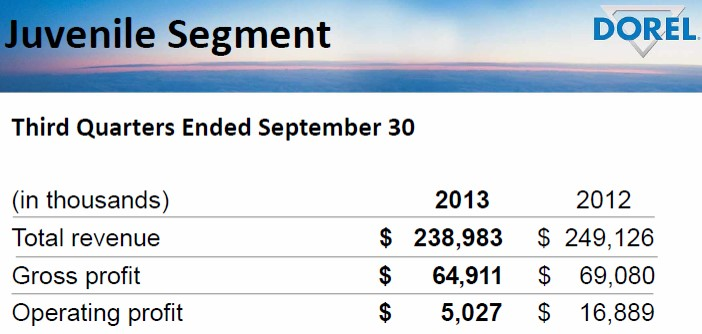
\includegraphics[scale=0.7]{juvenile}}
\centerline{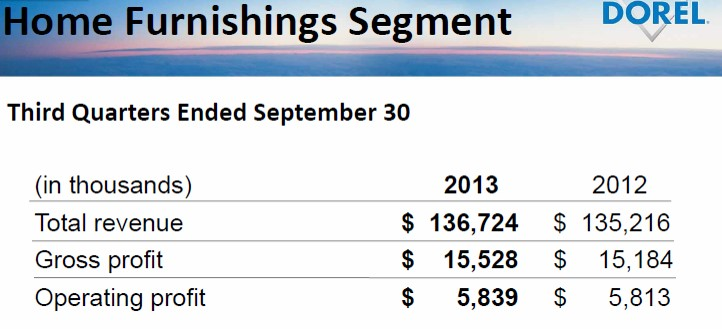
\includegraphics[scale=0.7]{furnishings}}
\centerline{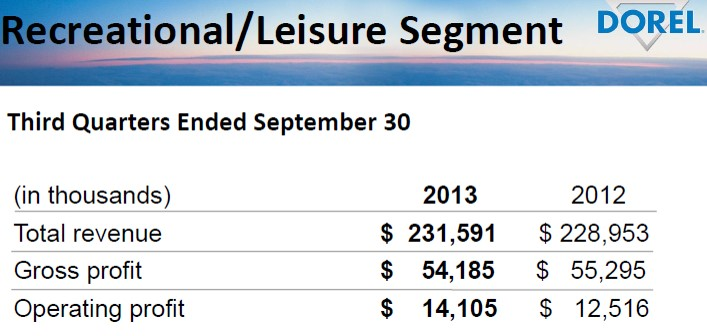
\includegraphics[scale=0.7]{recreational}}




%************************************************
\chapter{Competitive Strategy Analysis}
%************************************************








%************************************************
\chapter{Balanced Scorecard}
\label{chp:scorecard}
%************************************************
\centerline{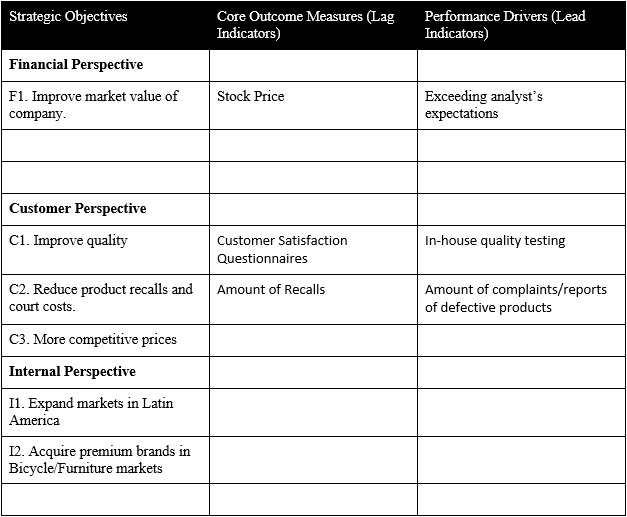
\includegraphics[scale=0.7]{scorecard}}

%************************************************
\chapter{SWOT Analysis}
\label{chp:swot}
%************************************************
\centerline{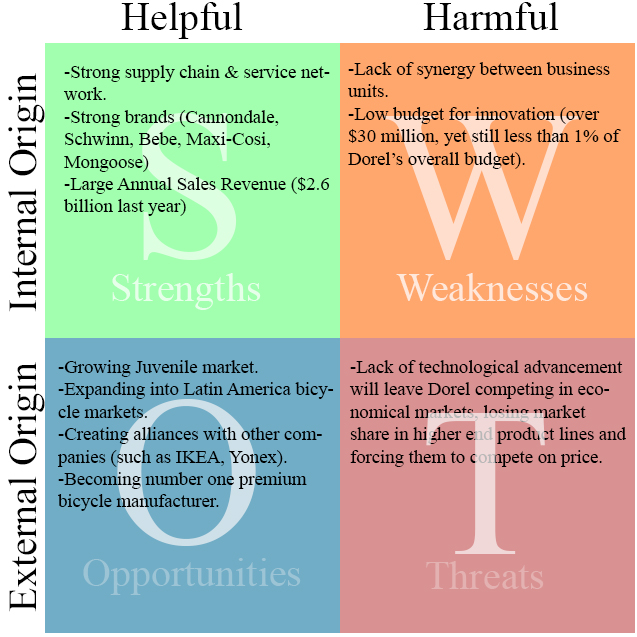
\includegraphics[scale=0.5]{SWOT}\index{SWOT}}

%************************************************
\chapter{Recommendations}
\label{chp:recommendations}
\index{Recommendations}
%************************************************
\section{Establish a BHAG}
While applying the five tests approach to Dorel, it became obvious that the largest issue facing the company is a lack of corporate vision.  At the moment, there is no overarching big hairy audacious goal that the company is seeking to accomplish.  We propose that Dorel establish a \index{BHAG}BHAG, which will help focus and direct the company, and help shape future decisions.  Based on market growth data, as well as Dorel's acquisitions, our suggested BHAG is to become the \index{World Leader}world's leader in premium bicycles.  

\subsection{International Premium Bicycle BHAG Roadmap}
\begin{enumerate}
  \item{Focos solely on the premium bicycle market.  Consider reversing plans to outsource bicycle production, bringing production back to the U.S. in order to improve quality. }
  \item{Increase R\&D expenditures, and market Dorel's more advanced product features such as the "Guru Fit System" \cite{Guru2014}.}
  \item{Instead of entering markets by acquiring additional brands, focus on improving and marketing one specific brand (we recommend Cannondale, as it has a strong reputation worldwide).  This will reduce unncessary \index{Acquisitions}acquisition costs, leaving more money to be invested in marketing and research.} 
\end{enumerate}

\section{Quality over Quantity}
\index{Quality over Quantity}We believe that in order to be successful, Dorel must return to its original core values of quality, safety, and value.  Currently, the company has drifted to a philosophy of cutting costs wherever possible, and only measuring success based on the current profit margin \cite{BRAINStaff2012}.  If Dorel continues down this path, it will lead to competing solely on price point, ironically still dropping \index{Profit Margins}profit margins.  We propose alternatively, that Dorel budget extensively for improving quality, which will in turn dramatically improve safety as well as increasing the \index{Value}value of its products.  This will make it easier to market those products, as well as increasing \index{Profit Margins}profit margins through \index{Brand Recognition}brand recognition.